\documentclass[conference]{IEEEtran}
\IEEEoverridecommandlockouts
% The preceding line is only needed to identify funding in the first footnote. If that is unneeded, please comment it out.
\usepackage{cite}
\usepackage{amsmath,amssymb,amsfonts}
\usepackage{algorithmic}
\usepackage{graphicx}
\usepackage{textcomp}
\usepackage{xcolor}
\def\BibTeX{{\rm B\kern-.05em{\sc i\kern-.025em b}\kern-.08em
    T\kern-.1667em\lower.7ex\hbox{E}\kern-.125emX}}
\begin{document}

\title{2024 FinTechIntro Final Research Report\\
        \normal {The Bonfire Wallet}}

\author{\IEEEauthorblockN{Allen Chen}
\IEEEauthorblockA{\textit{National Taiwan University} \\
Taipei, Taiwan \\
B10209040@ntu.edu.tw}
}

\maketitle

\begin{abstract}
This report is the final project of 2024 spring Introduction to FinTech. It will cover the 
current state and the future of the Bonfire wallet, such as its architecture and history. And 
comparisons of the existing burner wallets. Since the Bonfire wallet utilize WebAuthn, we will 
also investigate how does its verification system work. 

\end{abstract}

\begin{figure}[htbp]
    \centerline{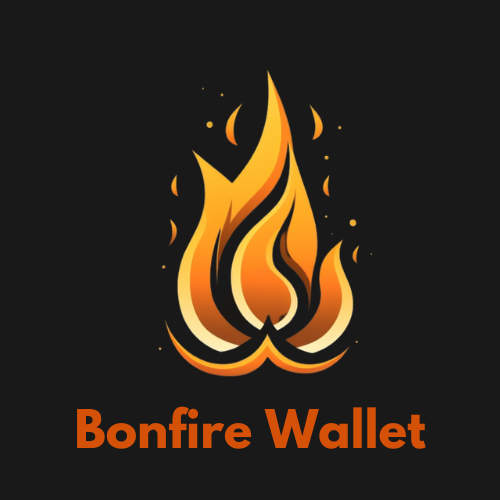
\includegraphics[width=150pt]{fig1.png}}\label{fig}
    \end{figure}


\section{Introduction}
The Bonfire wallet is a edge-cutting web application which allow users to create a burner wallet
using WebAuthn. WebAuthn is a web standard that belong to the FIDO2 project, and his project aims 
to standarlize an interface for authenticating users to web-based applications and services using 
public-key cryptography. Thus, with the integration of WebAuthn, users can create a passwordless 
wallet, increasing the level of security. 

\section{Background}

A \textbf{burner wallet}, or a "disposable wallet" as people would call it, is basically a crypto wallet 
that users create for potentially risky interactions with various blockchain applications. Under
the circumstance, this kind of wallet or account should not store large amount of crypto but 
should contain just enough for a single or a few interactions. One can create a burner wallet 
using hierarchical deterministic wallets (HD wallets), which are capable of generating numerous accounts
from a single secret seed phrase. 

\begin{figure}[htbp]
    \centerline{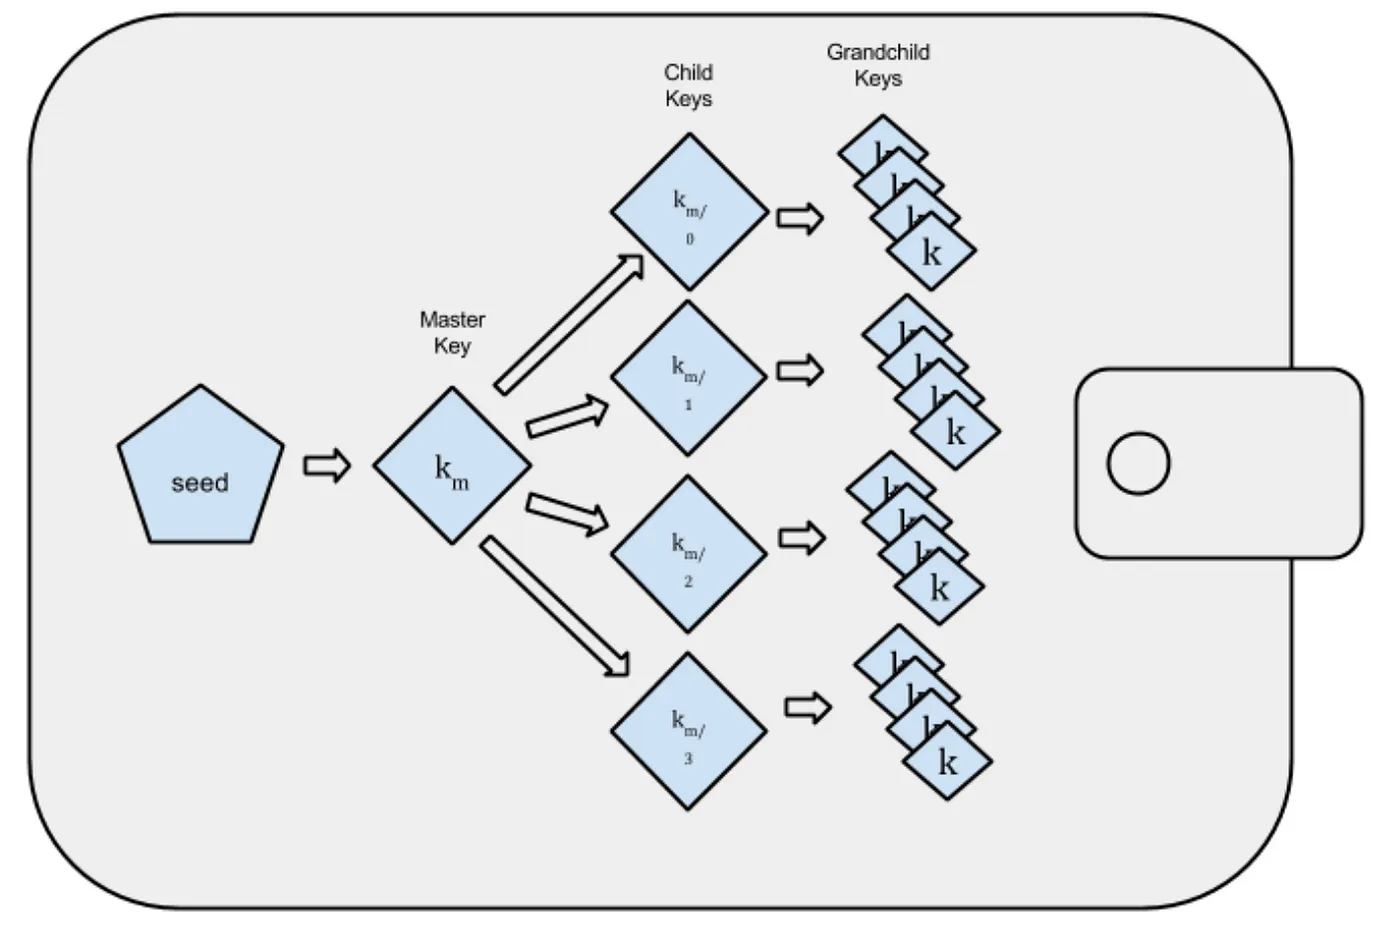
\includegraphics[width=250pt]{fig2.png}}\label{fig}
    \caption{The structure of HD wallet [1]}
    \end{figure}

As mentioned in the Introduction, \textbf{WebAuthn} makes people much more convenient to do their 
ID verification. Different from the traditional MFAs (Multi-Factor Authentication) such as text messages,
one-time password (OTP), PIN, and etc, WebAuthn possesses the ability to not to become a target for 
phishing attacks. And users don't need to fill in all their informations by hands, which does save much
time. 

\begin{figure}[htbp]
    \centerline{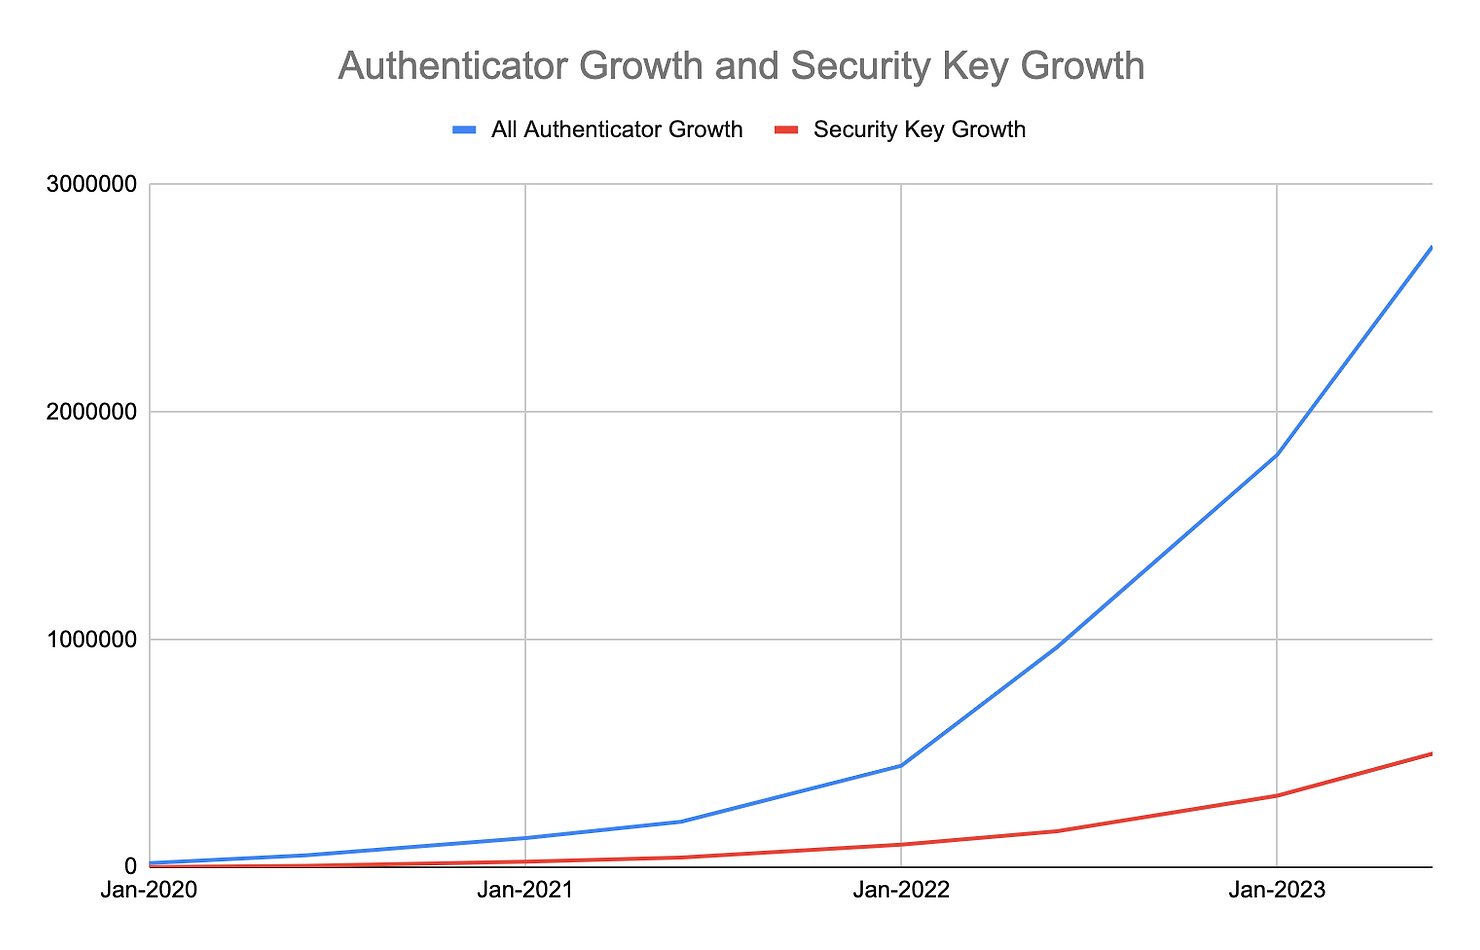
\includegraphics[width=250pt]{fig3.png}}\label{fig}
    \caption{The trend (blue line) shows WebAuthn's popularity among the field of ID verification [2]}
    \end{figure}

\section{The achiteture of Bonfire wallet}
Bonfire is built on RISC-Zero. It is the world's first zero-knowledge virtual machine which can run 
arbitrary code as a zero-knowledge proof. With the help of RISC-Zero, this web application will be 
able to offload the computation of the verification of the signature that WebAuthn provides  
after authenticating. Bonfire is consisted of two parts: the frontend web wallet and the solidity 
smart contract.  

\subsection{the Frontend}\label{AA}
Users are asked to register via WebAuthn in the browser. There are some options they can choose, for 
instance fingerprint, physical token, bluetooth device and more. Users who finish registration will
get their own public key. When it comes to making a transaction, the WebAuthn will come in handy 
again, and the transaction will be approved once the user authenticate in the same way that they registered.
Plus, this process will also generate a digital signature that using ECDSA with secp256r1 curve. It's 
based on the mathematical properties of elliptic curves and operates in a finite field over prime numbers, 
providing 256-bit security level, which means that it is resistant to attacks that try to solve the 
elliptic curve discrete logarithm problem with current computational capabilities.

\subsection{the Smart Contract}
A smart contract must be deployed with the creation of each new burner wallet. Within the smart contract
there is a public key that can uniquely identify the burner wallet (The address of the smart contract 
is the burner wallet's address). Another function of the smart contract is to handle the verification 
process, it will receive a WebAuthn signature that has to be verified in order to execute the transaction. 
Since the verication cost too much computational resource, this process will be offloaded to the Bonsai 
Proving Service, a service that uses a parallelized cluster to accelerate proving times. This way users 
don't have to generate proof on their own with slow speed. 

\begin{figure}[htbp]
    \centerline{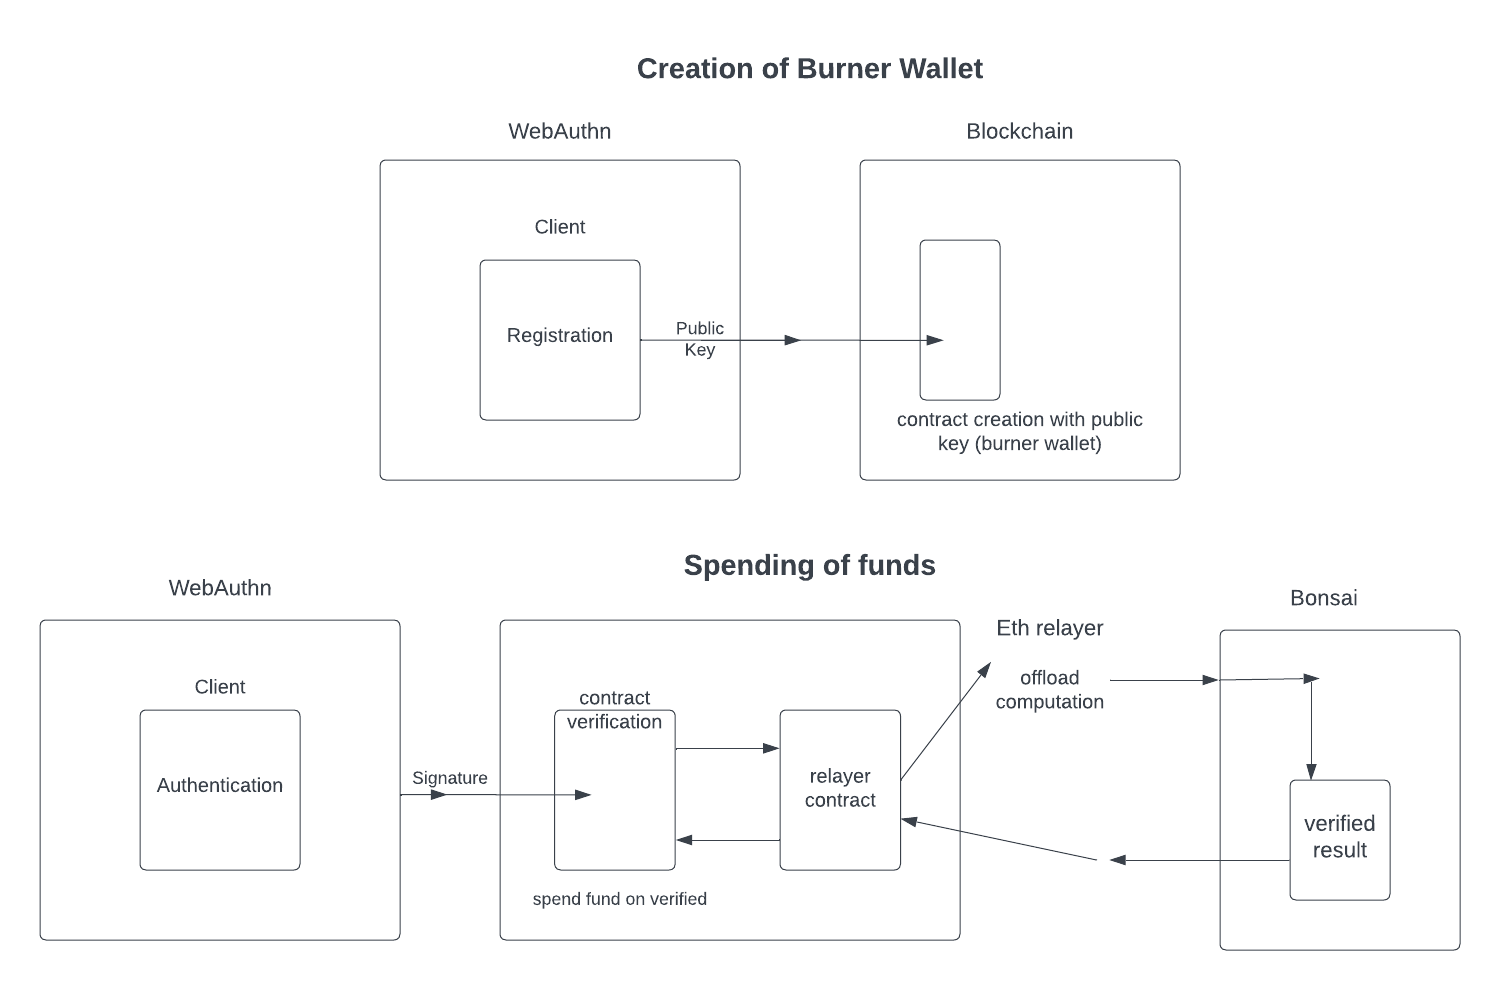
\includegraphics[width=250pt]{projects_n1dzp_images_Bonfire Wallet Diagram.png}}\label{fig}
    \caption{The structure of Bonfire wallet [3]}
    \end{figure}

\section{Existing Burner Wallet}
Due to the vitality of crptocurrency market, there are many kinds of burner wallet people use to store 
their crypto assets. 

\begin{table}[htbp]
    \caption{Comparison of Burner Wallets}
    \begin{center}
    \begin{tabular}{|c|c|c|}
    \cline{1-3} 
    \textbf{} & \textbf{\textit{Name}}& \textbf{\textit{Feature}} \\
    \hline
    \textbf{1.} & Bonfire & Passwordless Access\\
    \hline
    \textbf{2.} & Metamask & Browser Extention\\
    \hline
    \textbf{3.} & Rainbow & user-friendly Ethereum wallet\\
    \hline
    \textbf{4.} & Burner wallet$^{\mathrm{a}}$ & designed for quick use\\
    \hline
    \multicolumn{3}{l}{$^{\mathrm{a}}$The original wallet made by A. Griffith.}
    \end{tabular}
    \label{tab1}
    \end{center}
    \end{table}

\subsection{Metamask}
Metamask supports Ethereum and ERC-20 tokens, and it is a browser extention, which makes user easy to 
manage their crypto assets. It also integrates with all kind of decentralized applications. In fact 
Metamask is not a dedicated burner wallet, but it allows users to create temporary accounts that can 
be used and discarded quickly.

\begin{figure}[htbp]
    \centerline{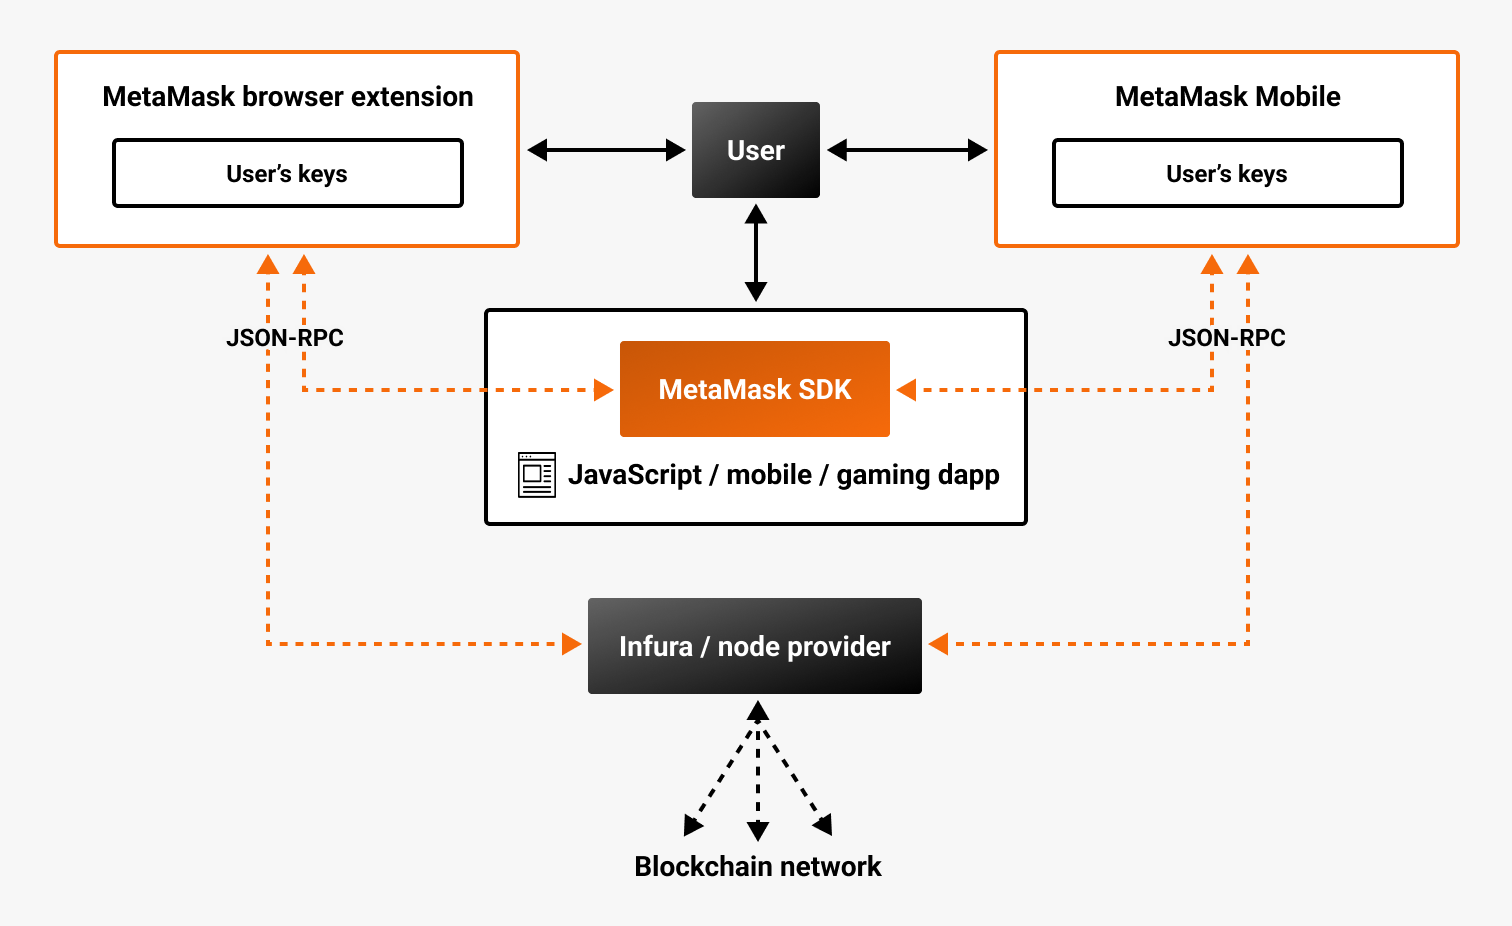
\includegraphics[width=250pt]{web3-architecture-692705a57011e90a523806281fdf2219.png}}\label{fig}
    \caption{The high-level architecture of the MetaMask web3 stack [4]}
    \end{figure}

\subsection{Rainbow}
Rainbow wallet focuses more on mobile users, and it's open source unlike most of other wallet applications
. In addition, the features it provides are convenient for managing NFTs, and users can use the application 
as if they are using social media APPs.

\subsection{Burner Wallet}\label{SCM}
The burner wallet developed by Austin Griffith is a web wallet which is made for moving small amount of 
crypto quickly. One can simply scan a QR code to send and receive funds along with a user-friendly interface.

\section{ERC-4337 and Burner Wallet}

ERC-4337, as known as Account Abstraction, is an ethereum standard that aims to revolutionize the way that 
user accounts are handled in the Ethereum ecosystem, as part of the Shenghai hard fork of the Shapella Upgrade.\\
In most blockchain system, users manage their transactions through Externally Owned Accounts (EOAs). These accounts
require them to own private keys and use them to process each transaction, thus the security and usage complexity 
issues would be raised. \\
By adopting account abstraction, users don't need to depend on EOAs anymore. Instead, the concept embeds smart 
contracts in user's wallet, therefore all actions can be done autommatically.\\
As a result, EOA wallets such as Metamask are facing the problems of low execution efficiency. For example, only ETH
can be used as Gas Fee, and if the wallet has no ETH, no transactions can be conducted; every action requires re-signing
, and so on.\\

\begin{figure}[htbp]
    \centerline{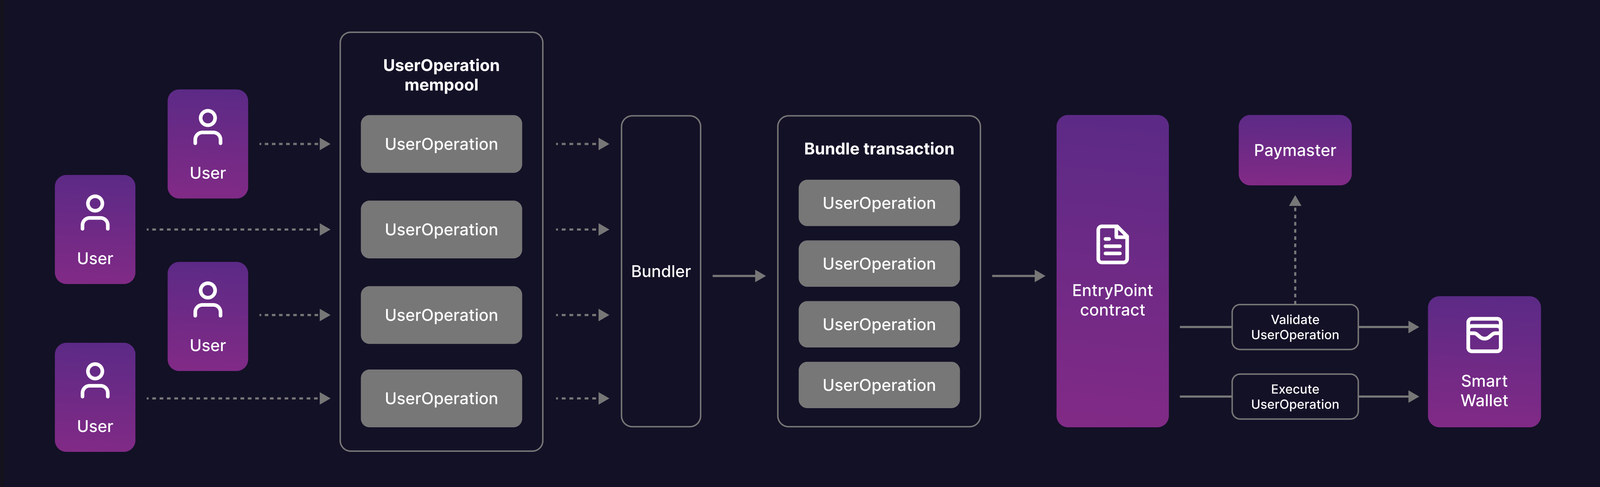
\includegraphics[width=250pt]{How-transactions-work-in-Ethereum-Smart-Accounts---ERC-4337-Account-Abstraction.png}}\label{fig5}
    \caption{How transactions work in Ethereum smart accounts [5]}
    \end{figure}

From Fig.5 we can clearly see the whole workflow of a smart contract wallet. The UserOperation mempool 
collects these transactions before they are processed. This is similar to the regular transaction pool in Ethereum 
but specific to user operations under ERC-4337. The Bundler collects multiple UserOperations from the mempool. 
These operations are then bundled together into a single Bundle transaction. The EntryPoint contract acts as the 
central component for processing the bundled transactions, for it validates and executes the operations contained in 
the bundle.

\section{Conclusion}
Burner wallets are perfect applications for one-time transaction or other purposes, such as NFT minting. However, the 
common burner wallets like Metamask involve too many steps of verification and confirmation. In order to simplify those 
Preparatory works, the Bonfire Wallet came on the scene. With WebAuthn, this web application is able to speed up the 
transaction process while ensuring user's account security. Along with ERC-4337 the ecosystem of Ethereum might be
changed significantly.


\begin{thebibliography}{00}
\bibitem{b1} https://medium.com/@bun919tw/hd-wallet-970096a6d72f
\bibitem{b2} https://www.odin-info.com.tw/post/webauthn-growth-and-challenges
\bibitem{b3} https://ethglobal.com/showcase/bonfire-wallet-n1dzp
\bibitem{b4} https://docs.metamask.io/wallet/concepts/architecture/
\bibitem{b5} https://blog.thirdweb.com/account-abstraction-erc4337/\\
 \\
https://www.lcx.com/smart-contract-wallet-explained/\\
 \\
STOICA, Gabriel-Marius. "Account Abstraction on Ethereum."\\
 \\
Onica, Emanuel, and Marius Georgică. "Can Smart Contracts Become Smart? An Overview of Transaction Impact on 
Ethereum DApp Engineering." 2023.\\
 \\
Lee, Wei-Meng. "Using the MetaMask crypto-wallet." Beginning Ethereum Smart Contracts Programming: With Examples 
in Python, Solidity, and JavaScript. Berkeley, CA: Apress, 2023. 111-144.\\
 \\
OpenAI. (2024). ChatGPT (Jun 8 version) [Large language model].
\end{thebibliography}

\end{document}
